\documentclass[10pt,twocolumn]{article}
\usepackage[letterpaper,top=0.64in,bottom=0.68in,left=0.66in,right=0.66in,columnsep=0.24in]{geometry}
\usepackage[T1]{fontenc}\usepackage{lmodern}\usepackage{microtype}\usepackage{graphicx}\usepackage{booktabs}
\usepackage{array}\usepackage{caption}\usepackage{xcolor}\usepackage{enumitem}\usepackage{tikz}
\usepackage{balance}
\usetikzlibrary{positioning}
\usepackage[hidelinks]{hyperref}\usepackage{url}
\definecolor{sprited}{HTML}{6337C7}\definecolor{teal}{HTML}{008C95}\definecolor{pale}{HTML}{F3F0FA}\definecolor{muted}{HTML}{555555}
\hypersetup{colorlinks=true,linkcolor=sprited,citecolor=sprited,urlcolor=sprited,
pdftitle={Dancing Stick Figures: A Synthetic Video Dataset, Renderer, and Diagnostic Evaluation Suite},
pdfauthor={Jin Hyuk Cho},pdfsubject={Synthetic video dataset, renderer, and diagnostic evaluation suite},
pdfkeywords={video generation, benchmark, synthetic dataset, structural evaluation, education}}
\captionsetup{font=small,labelfont=bf,skip=4pt}\setlist{nosep,leftmargin=*}
\setlength{\parindent}{1em}\setlength{\parskip}{0pt}\setlength{\textfloatsep}{8pt plus 2pt minus 2pt}
\setlength{\floatsep}{7pt plus 2pt minus 2pt}\setlength{\intextsep}{7pt plus 2pt minus 2pt}\renewcommand{\arraystretch}{1.08}

\title{\vspace{-1.5em}\textbf{Dancing Stick Figures: A Synthetic Video Dataset,\\Renderer, and Diagnostic Evaluation Suite}}
\author{Jin Hyuk Cho\\Sprited\\\small\href{mailto:jin@sprited.ai}{jin@sprited.ai} $\cdot$
\href{https://orcid.org/0009-0001-1896-8242}{ORCID 0009-0001-1896-8242}\\[-2pt]
\small\href{https://huggingface.co/datasets/sprited/dancing-stick-figures}{Dataset} $\cdot$
\href{https://github.com/sprited-ai/dancing-stick-figures}{Code} $\cdot$
\href{https://huggingface.co/sprited/dancing-stick-figures-baselines}{Models} $\cdot$
\href{https://colab.research.google.com/github/sprited-ai/dancing-stick-figures/blob/main/notebooks/dancing_stick_figures_colab_v0_3.ipynb}{Colab}}
\date{}

\begin{document}\raggedbottom\maketitle\vspace{-1.25em}
\begin{abstract}
End-to-end study of video generation---training a model, inspecting its samples, and explaining its
failures---faces three practical obstacles: datasets are large, real video has no answer key,
and aggregate scores do not say why a video failed. \textbf{Dancing Stick Figures} is a synthetic video dataset
with a deterministic renderer, built so that the whole experiment fits on one GPU. It contains 1,340 six-second motions rendered from three cameras. Every frame stays linked to
the joints, camera, body parameters, depth, surface normals, part labels, and source motion that produced it,
so evaluation has an answer key. Rule-based measurements check whether coloured limbs stay connected and how
position and pose change over time. Controlled corruptions test what each measurement can and cannot see: in a
120-frame study, playing videos backward leaves the time-symmetric motion signals unchanged and scores FVD 79.3
where real--real scores 80.5. The release includes a 0.79-GB $64^2$ training tier, fixed evaluation manifests,
checkpoints, and a Colab lesson.
\end{abstract}

\section{Introduction}
Strong video generation systems such as Seedance and MiniMax H3~\cite{gao2025seedance,minimax2026h3} publish
results and sometimes weights, yet access to those artifacts is not the same as the ability to study them.
Three barriers separate the two:
\begin{itemize}[leftmargin=*,nosep]
\item \textbf{Data.} The exact data, filters, and recipe behind a strong model are rarely released together,
so a failure cannot be traced back to what the model saw.
\item \textbf{Experimentation.} Frontier training needs large corpora, heavy compute, and pretrained codecs.
What stays affordable is prompting and fine-tuning, not retraining a controlled variant.
\item \textbf{Evaluation.} ``Better'' can mean cleaner frames, an intact body, plausible motion, or prompt
adherence; these change independently, and an aggregate score does not say which one changed.
\end{itemize}

The question this paper addresses is practical: can someone with a single GPU train video generation models
from scratch on a small but meaningful dataset, and study their behaviour through repeated, controlled
experiments? That requires the full image-to-video path to fit one consumer GPU or a Colab runtime, a run to
produce inspectable multi-second samples in hours, and evaluation that measures visible failures directly,
with known blind spots.

Dancing Stick Figures is built to those constraints: a dataset and renderer whose frames stay connected to
their generating state, an evaluation suite whose measurements are themselves tested, and reference models
with a Colab workflow that runs the whole path.

The release contributes:
\begin{enumerate}
\item a label-rich video dataset with a 0.79-GB $64^2$ tier, an optional $32^2$ tier, the motion, camera, and
body parameters behind every frame, and a deterministic renderer;
\item a seed-disjoint evaluation protocol, structural evaluator, and controlled corruption suite; and
\item image and video trainers, checkpoints, and an end-to-end Colab curriculum.
\end{enumerate}

\begin{figure*}[t]\centering
\resizebox{\textwidth}{!}{%
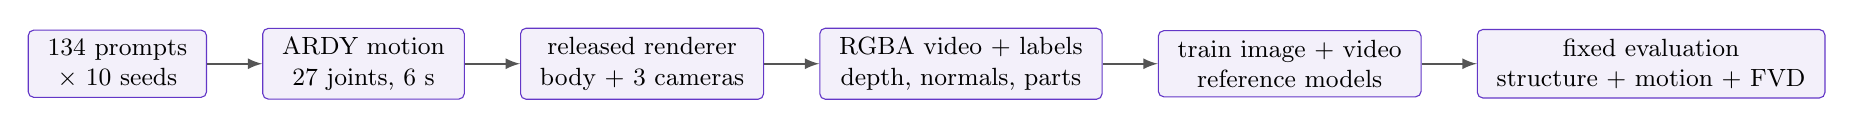
\begin{tikzpicture}[font=\small,node distance=5mm and 7mm,
box/.style={draw=sprited,rounded corners=2pt,fill=pale,align=center,minimum height=8mm,inner xsep=7pt},
arr/.style={-latex,thick,draw=muted}]
\node[box] (prompt) {134 prompts\\$\times$ 10 seeds};
\node[box,right=of prompt] (motion) {ARDY motion\\27 joints, 6 s};
\node[box,right=of motion] (render) {released renderer\\body + 3 cameras};
\node[box,right=of render] (data) {RGBA video + labels\\depth, normals, parts};
\node[box,right=of data] (train) {train image + video\\reference models};
\node[box,right=of train] (eval) {fixed evaluation\\structure + motion + FVD};
\draw[arr] (prompt)--(motion);\draw[arr] (motion)--(render);\draw[arr] (render)--(data);
\draw[arr] (data)--(train);\draw[arr] (train)--(eval);
\end{tikzpicture}}
\caption{From source motion to diagnosis. Every rendered frame stays linked to the motion, camera, body, and
buffers that generated it.}\label{fig:loop}
\end{figure*}

\section{Related Work}
Several lines of work provide synthetic video, human-motion supervision, or decomposed evaluation; none
packages them as one experiment a reader can rerun and alter.

\paragraph{Small and controlled video.} Moving MNIST~\cite{srivastava2015unsupervised} made temporal prediction
cheap, but has no articulated structure or language conditioning. Kubric and MOVi~\cite{greff2022kubric} showed
the value of programmable rendering with dense ground truth for scene understanding. Neither offers a compact
route from text-conditioned generator training to failure diagnosis. We restrict the scene to one articulated
figure so that the whole route stays small enough to rerun.

\paragraph{Synthetic people.} SURREAL~\cite{varol2017surreal} and BEDLAM~\cite{black2023bedlam} render large,
realistic human datasets and ask whether synthetic people can train perception systems. We ask a different
question with a much smaller dataset: whether a reader can train a video generator from scratch, observe its
failures, and relate them back to known motion and rendering state.

\paragraph{Training data for video generation.} HumanVid~\cite{wang2024humanvid} and
MiraData~\cite{ju2024miradata} improve the coverage and transparency of video training data at scale. They do
not aim to make pretraining itself a short experiment. Our 0.79-GB tier makes the opposite trade: narrow visual
scope for a pipeline that can be inspected end to end. Synthetic data has also been used to improve large
generators directly~\cite{zhao2025synthetic,jin2026dynavid}; those works target a different compute regime, one
where the reader inherits a large pretrained model rather than training the generator themselves.

\paragraph{Human motion as source data.} AMASS~\cite{mahmood2019amass} and HumanML3D~\cite{guo2022humanml3d}
support motion modelling without a pixel renderer or visual evaluation; we use articulated motion as source
material and simplify appearance so generated pixels can be related to joints and limbs.

\paragraph{Evaluation of generated video.} FVD~\cite{unterthiner2018fvd} is a useful distributional distance,
but it responds more to frame content than to temporal corruption~\cite{ge2024fvdbias}. T2V-CompBench and
VBench-2.0~\cite{sun2025compbench,zheng2025vbench2} decompose quality into many axes; GeneVA~\cite{kang2026geneva}
and Ref4D-VideoBench~\cite{wei2026ref4d} localise artifacts with human or reference supervision. We work in one
fully specified domain instead, where controlled mistakes show exactly which signals react and which do not.
This complements semantic, perceptual, and human evaluation; it does not replace them.

\section{Dataset and generation pipeline}
We generated one motion per seed 0--9 for each of 143 prompts in six groups (dance, gesture, locomotion,
transition, idle, sport) with NVIDIA ARDY~\cite{zhao2026ardy}. Each motion is six seconds at 20 fps. A
z-buffered capsule renderer with $4\times$ supersampling emits three deterministic orthographic views. Nine
prompts were removed by visual curation because their motions do not visibly perform the requested action in
this domain, for example \emph{shakes their head no} (the head is a filled circle), \emph{push up} (the action
does not appear), and \emph{climbs over a low wall} (the wall does not exist in the render). The release
contains 134 prompts; the exclusion list ships with per-prompt reasons. Prompts whose stillness is correct (the
idle group) are kept even when the low-motion QA flag fires. Table~\ref{tab:data} summarises the data. Seeds
0--7 train, seed 8 validates, seed 9 tests: every prompt appears in all three splits, and no source motion
crosses a split boundary (Table~\ref{tab:splits}).

\begin{table}[t]\centering\caption{Released data. A motion is rendered from three views.}\label{tab:data}\small
\begin{tabular}{@{}lrrr@{}}\toprule Configuration & Rows & Resolution & Size \\\midrule
\texttt{frames} & 482,400 & $128^2$ & 4.4 GB \\
\texttt{mini} & 482,400 & $64^2$ & 0.79 GB \\
\texttt{motion} & 1,340 & 27 joints & 0.33 GB \\\bottomrule\end{tabular}\end{table}

\begin{table}[t]\centering
\caption{Seed-disjoint splits. Each split contains all 134 prompts; source motions are disjoint by seed.}
\label{tab:splits}\scriptsize
\begin{tabular}{@{}lrrrr@{}}\toprule
Split & Prompts & Motions & Videos & Frames \\\midrule
Train & 134 & 1,072 & 3,216 & 385,920 \\
Validation & 134 & 134 & 402 & 48,240 \\
Test & 134 & 134 & 402 & 48,240 \\
All & 134 & 1,340 & 4,020 & 482,400 \\\bottomrule
\end{tabular}
\end{table}

\begin{figure*}[t]
\centering

\includegraphics[width=\textwidth]{paper/figs/dataset_anatomy.pdf}
\caption{One released motion viewed through the dataset. (b) Five frames at equal increments of pose-space
motion, so an idle tail cannot dominate the strip. (a) The middle pose from the clip's three cameras. (c) The
same frame with part segmentation, depth, camera-space normals, and projected joints. Each record also stores
its prompt, source-motion identifier, seed, camera, and body parameters.}
\label{fig:dataset-anatomy}
\end{figure*}

The generator samples limb length, scale, stroke, and camera yaw and pitch deterministically from
\texttt{clip\_id}. It stores 3D and projected joints, visibility, camera and body parameters, RGBA, 16-bit
depth, camera-space normals, 27-part segmentation, and the raw motion (Figure~\ref{fig:dataset-anatomy}). The
domain uses one visual style, one figure per frame, orthographic cameras, and at most $128^2$ resolution. The
builder records two motion-quality flags (\texttt{frozen}, \texttt{levitation}); flagged samples stay in the
release so filtering choices are explicit.

The configurations are compute tiers of one dataset. $128^2$ keeps the most detail; the 0.79-GB $64^2$ tier is
the primary training tier; $32^2$ supports smoke tests. Reported structural results use $64^2$, where the thin
coloured limbs remain measurable. The motion release supports rebuilding the full visual dataset without ARDY;
\S\ref{sec:access} describes the rebuild and its verification.

\section{Tasks and failure diagnostics}
\paragraph{Video task.} Each clip has 120 frames at 20 fps, and dataset-level evaluation uses the complete
clip. The reference models train on a declared window view: the first 64 frames of each clip (3.2 seconds).
This restriction keeps the training tensor within one GPU and concentrates training where the prompted action
occurs, because ARDY does not pace an action to the requested duration and later frames often idle. The window
rows in Table~\ref{tab:backbone-results} compare generated 64-frame windows with real windows drawn under the
same manifest rule.

\paragraph{Structural answer key.} Each arm and leg uses a fixed pair of colours. The evaluator converts a
frame into eight limb-colour masks and reports:
\begin{itemize}\setlength\itemsep{0pt}
    \item \textbf{Topology violation rate (TVR):} limb colours missing or split into multiple components;
    \item \textbf{Limb-identity error (LIE):} expected colour adjacencies that are absent;
    \item \textbf{Colour-purity error (CPE):} foreground pixels outside the rendering palette;
    \item \textbf{Foreground fraction:} pixels occupied by the figure; and
    \item \textbf{Clean rate:} frames with both TVR and LIE at zero.
\end{itemize}
For video, it adds colour-mass drift, centroid speed and acceleration, motion fraction, angular speed and
jerk, and height variation. These are image-space diagnostics, not biomechanics. The motion quantities are
two-sided reference signals: zero can mean a stopped video, and large values can mean jitter. Agreement with
the real reference, not a small value, is the target.

Occlusion produces non-zero topology scores even on ground-truth renders, so ground-truth scores are a
\emph{real reference}, not an error floor. A deterministic manifest selects one camera per source motion and
keeps the two 128-video reference halves motion-disjoint. For FVD~\cite{unterthiner2018fvd} we composite RGBA
onto white, resize to $224^2$, and extract I3D features; values are comparable only within this fixed
implementation and sample count.

\paragraph{Controlled validation.} Five deterministic structural corruptions were applied to 500 held-out
rerenders. A partial left/right limb swap raises LIE by .203; an extra arm raises TVR by .085. A whole-limb
swap preserves the colour graph and is not detected; bone stretching and hand deletion are also missed, because
the metrics measure topology, not proportions or end-effectors. Temporal corruptions (freeze, shuffle, loop,
reverse) are evaluated in \S\ref{sec:results}.

\begin{figure*}[t]\centering

\includegraphics[width=0.96\textwidth]{paper/figs/failure_modes.pdf}
\caption{Controlled study on complete six-second clips ($n=128$ per set). \emph{Freeze} repeats frame 1,
\emph{shuffle} permutes all 120 frames, \emph{reverse} plays them backward, \emph{first 8 looped} repeats
frames 1--8. (a) Freezing zeroes the motion signals; shuffling and looping create excess acceleration and
angular jerk; reversal changes neither. (b) Against the 80.5 real--real reference, FVD responds to freezing,
shuffling, and looping, but scores reversed video at 79.3.}
\label{fig:failures}\end{figure*}

\section{Diagnostic validation and reference results}\label{sec:results}

\paragraph{Metric stress test.} Figure~\ref{fig:failures} reports the 120-frame study. The two real sets have
centroid speeds .313 and .299 pixels per frame. Freezing zeroes all motion signals. Shuffling raises centroid
acceleration from .348 to 2.858 and angular jerk from .060 to .384; looping raises them to .507 and .084.
Reversal changes neither the frame set nor any reported motion signal, and FVD scores it 79.3 against the real
reference's 80.5 (freeze 465.5, shuffle 419.2, loop 328.5). Across 30 paired 64-video trials, reversal changes
FVD by $-1.65\pm2.69$. Reversal is a shared blind spot: the hand-designed signals are time-symmetric by
construction, and FVD does not see it either. Neither measurement certifies directionally correct motion.

\paragraph{Released reference models.} The reference experiments form a ladder that changes one variable per
rung. The shared backbone is a 39.9M-parameter factorised video DiT: $4\times4$ frame patches, alternating
spatial and temporal attention blocks, flow-matching velocity prediction (a linear interpolant; often called
rectified flow, though we apply no reflow step)~\cite{peebles2023dit,lipman2023flow}, and a frozen T5-small
encoder attached through cross-attention. With $T{=}1$ the network is an image generator; with $T{=}64$ it
generates the full training window jointly.

The first rung is initialisation: the 64-frame model trains from random weights and, separately, warm-started
from the image checkpoint's spatial and text weights. Image-first initialisation is established
practice~\cite{ho2022vdm,singer2023makeavideo}; the two rows are reference points, and the random row is the
matched comparator for the latent rows. The second rung varies the mechanism that carries motion across patch
boundaries: the factorised baseline, a zero-initialised local $3{\times}3{\times}3$ convolutional mixer added
to every block, and joint attention over all spatio-temporal tokens. These are measured at pixel scale with the
same warm start; joint attention costs $4.7\times$ the factorised step in wall-clock. The latent block repeats
the two attention extremes where 1{,}024 tokens make them nearly cost-matched (0.17 vs.\ 0.19\,s/step). The
third rung varies representation: matched DiTs trained in the latent space of a separately trained frozen video
autoencoder, decoded before evaluation, with a codec-floor row (real windows encoded and decoded by the same
codec) to separate codec cost from model skill.

The codec predates the v0.2 curation and split, and a post-hoc audit found two defects: it reconstructs
training foregrounds with $63\%$ lower masked error than held-out foregrounds, and neutralising its background
latent cells degrades foreground reconstruction $33\times$ (a re-trained reference codec: $3$--$5\times$). The
codec memorised training clips and stores foreground information in background latents. The latent rows
therefore illustrate the representation axis under a weak codec; they do not bound what latent training can
reach. Re-trained codecs that pass this audit (held-out gap ${\approx}10\%$) are planned for a revision.

Table~\ref{tab:backbone-results} collects the runs. Each block names its protocol, because single-frame and
64-frame scores are different measurements. Earlier v0.1 baselines remain released but were trained under a
superseded split and are not comparable rows. Figure~\ref{fig:dit-samples} shows the warm-started model.

\begin{table*}[t]
\centering
\caption{Reference ladder on the released seed-disjoint data. Every model trains on the same $64^2$ cache and
first-64-frame view with the same flow-matching trainer, optimiser, and step budget; one variable changes per
rung. Rows are comparable only within a protocol block. ``Image'' initialisation copies compatible spatial and
text weights from the single-frame checkpoint.}
\label{tab:backbone-results}
\scriptsize
\setlength{\tabcolsep}{3.8pt}
\begin{tabular}{@{}lllrrrrrrrr@{}}\toprule
Model & Attention & Init. & TVR$\downarrow$ & LIE$\downarrow$ & CPE$\downarrow$ & Speed & Motion frac. & Jerk & FVD$\downarrow$ \\\midrule
\multicolumn{10}{@{}l}{\textit{Single frames, prompt-conditioned, $n=512$, 50 sampling steps}}\\
Real validation frames & --- & --- & .115 & .093 & .039 & --- & --- & --- & --- \\
Image DiT, 30k & factorised & random & .128 & .050 & .030 & --- & --- & --- & --- \\
\addlinespace
\multicolumn{10}{@{}l}{\textit{64-frame windows at 20 fps, prompt-conditioned, $n=128$ held-out source motions}}\\
Real reference windows & --- & --- & .116 & .093 & .037 & .373 & .501 & .073 & 115.2 / ref. \\
Codec reconstruction floor & --- & --- & .137 & .104 & .037 & .380 & .503 & .104 & 124.4 \\
Video DiT, 10k & factorised & random & .942 & .035 & .051 & .408 & .559 & .326 & 1641.3 \\
Video DiT, 10k & factorised & image & .169 & .045 & .034 & .850 & .719 & .324 & 545.0 \\
Video DiT, 10k & factorised + local mixer & image & .158 & .045 & .032 & .515 & .609 & .205 & 407.0 \\
Video DiT, 10k & joint spatio-temporal & image & .240 & .065 & .035 & .556 & .610 & .221 & 558.9 \\
Latent video DiT, 10k & factorised & random & .816 & .398 & .084 & .571 & .647 & .276 & 503.3 \\
Latent video DiT, 10k & joint spatio-temporal & random & .821 & .408 & .087 & .564 & .635 & .273 & 527.2 \\\bottomrule
\end{tabular}
\par\vspace{2pt}\raggedright\scriptsize TVR is topology violation rate, LIE limb inconsistency error, CPE
colour-purity error. Speed, motion fraction, and jerk are two-sided signals: agreement with the real row is the
target. The codec-floor row passes the real windows through the frozen autoencoder used by the latent rows;
latent scores should be read against it. Real training-split windows score FVD 125.7 against the same
reference, which is also what a training-set replay would score, so models near this band need a memorisation
check. A training-seed repeat of the warm-started video row scores TVR .183 / FVD 570.7 against .169 / 545.0.
\end{table*}

\paragraph{Reading the ladder.} Initialisation dominates at this budget. From random weights the 10k-step video
model violates topology in $94\%$ of frames (TVR .942, FVD 1641); warm-started, the same model reaches TVR .169
against .116 real. The seed repeat (.183, 570.7) shows these contrasts are large against training-seed
variance. The two measurement families also disagree in opposite directions. The warm-started pixel model has
near-real structure but too much motion (centroid speed .850 vs.\ .373 real), which FVD punishes. The latent
rows are the opposite: FVD near 500, TVR above .8, broken figures rendered smoothly by the codec. Ranking by
TVR alone and by FVD alone gives opposite orderings. The mixing rung also orders cleanly: the local mixer
improves on the factorised baseline in structure and motion at once (TVR .158 vs.\ .169, centroid speed .515
vs.\ .850, FVD 407 vs.\ 545), while joint attention, at $4.7\times$ the step cost, is worse on every measure
(TVR .240, FVD 559). Direct neighbour connectivity helps when it is nearly free; global connectivity does not
pay for itself within this step budget.
Changing the prompt under fixed noise has a measurable effect, and the paired wave examples in
Figure~\ref{fig:dit-samples} move the requested arm. This is bounded evidence of conditioning, not a calibrated
prompt-adherence score.

\begin{figure*}[t]
\centering

\includegraphics[width=\textwidth]{paper/figs/reference_generation_pairs.pdf}
\caption{Released clips and 10k-step DiT samples. Each block interleaves four time points from a released clip
and a generation (50 Euler steps, guidance 3). The paired wave prompts check laterality; running and backward
walking show locomotion under independently seeded noise.}
\label{fig:dit-samples}
\vspace{-3pt}
\end{figure*}

\paragraph{Why pixel space.} At $32^2$--$64^2$, pixel-space training is practical and keeps thin-limb errors in
the representation the evaluator scores. A separately trained video VAE adds a training stage and can confound
generator errors with codec artifacts, as the audited codec above shows. The core Colab therefore follows the
pixel-space route.

\section{Accessibility and reproducibility}\label{sec:access}
The repository releases the generator, cache builder, trainers, sampling code, evaluator, corruptions, FVD
evaluation, checkpoints, and comparison script. The notebook inspects the data, builds a cache, trains the
image generator, transfers its spatial weights, trains the video generator, samples a multi-second GIF, and
compares scores against real references. $32^2$ is a smoke test; $64^2$ is the reference exercise. Each stage
leaves an inspectable artifact before the next begins.

The motion release supports a full rebuild. The rebuild script recomputes body and camera settings from each
\texttt{clip\_id} and reruns the public renderer; ARDY is not required. The verifier was run over all 514,800
$128^2$ frames of the pre-curation generation: every motion and metadata label matches; colour and segmentation
pixels agree on 99.88\% and 99.92\% of comparisons; joint visibility, the least stable field, agrees on
99.50\%; depth and normals exceed 99.99\%. An independent $64^2$ rebuild passes with similar agreement. The
same script can rerender with seeded overrides to body scale, stroke, or camera, and the manifest records the
overrides; an instructor keeps the private seed for a course-specific rendering.

Resource cost decides who can run the experiment, so we report it with the results. On the ladder's GPU
(NVIDIA RTX PRO 6000 Blackwell, 96\,GB): the 30k-step image stage runs at 0.10\,s/step with a 10.5\,GB peak;
each 10k-step 64-frame video run peaks below 10\,GB with gradient checkpointing and fits a 12\,GB consumer
card. Measured step times are 3.4\,s for the factorised run (two runs sharing the GPU) and 1.07\,s for the
local-mixer run (exclusive). Disabling checkpointing raises the local-mixer peak to 55.1\,GB and lowers its
step to 0.82\,s; that trade only pays on large workstation cards. Step times transfer across GPUs only
approximately. An earlier UNet lesson completed on a hosted Tesla T4; hardware numbers are reported for the
hardware they were recorded on.

Our code is MIT and the dataset is CC0-1.0. Motions were generated with ARDY's 20-fps Core model (checkpoint
revision not retained). ARDY's code is Apache-2.0; its checkpoints are distributed under the
\href{https://www.nvidia.com/en-us/agreements/enterprise-software/nvidia-open-model-agreement/}{NVIDIA Open
Model Agreement}, which permits derivative works and claims no ownership of outputs.

\section{Limitations and next evaluations}\label{sec:future}
The domain is narrow by design: one raster style, one figure, orthographic cameras, no real-video proxy. The
colour-based evaluator measures visible topology, not bone length, joint angles, left/right semantics, or
biomechanics. The motions inherit ARDY's capabilities and biases, and we have not human-validated every
remaining motion. The seed-disjoint test measures in-domain generation under unseen motion realisations, not
zero-shot prompts or human motion at large. The colour metrics do not establish prompt adherence. Three
sampling seeds quantify generation noise for one checkpoint, not training variation or scaling.

The most direct extension is a learned rig estimator: map a generated video back to a rig, re-render it, and
compare, exposing rig-space failures such as unstable bone length or foot contact. Its scores would need
validation on controlled malformations before use as evidence.

\section{Conclusion}
Dancing Stick Figures makes a complete video-generation experiment small enough to run and concrete enough to
inspect. The released workflow trains an image generator, warm-starts a video generator from it, samples
multi-second videos, and connects visible failures to measurements of body-part connectivity and motion.
Controlled mistakes show why the measurements must be read together: the structural signals miss reversed time,
and FVD does not name the property that failed. It is a small, complete first experiment in video generation.

\paragraph{Use of AI systems.} The source motions were generated with ARDY's 20-fps Core model
(\S\ref{sec:results}); rendering, curation, and verification are deterministic code. An AI coding assistant
(Claude) was used for experiment orchestration, evaluation tooling, and manuscript editing under author
direction. All numerical results come from the released code and were reviewed by the author.

\balance
\begin{thebibliography}{99}\footnotesize
\setlength{\itemsep}{0pt}
\setlength{\parskip}{0pt}
\bibitem{srivastava2015unsupervised} N. Srivastava et al. Unsupervised Learning of Video Representations using LSTMs. \emph{ICML}, 2015.
\bibitem{greff2022kubric} K. Greff et al. Kubric: A Scalable Dataset Generator. \emph{CVPR}, 2022.
\bibitem{varol2017surreal} G. Varol et al. Learning From Synthetic Humans. \emph{CVPR}, 2017.
\bibitem{black2023bedlam} M. J. Black et al. BEDLAM: A Synthetic Dataset of Bodies Exhibiting Detailed Lifelike Animated Motion. \emph{CVPR}, 2023.
\bibitem{wang2024humanvid} Z. Wang et al. HumanVid: Demystifying Training Data for Camera-controllable Human Image Animation. \emph{NeurIPS Datasets and Benchmarks}, 2024.
\bibitem{ju2024miradata} X. Ju et al. MiraData: A Large-Scale Video Dataset with Long Durations and Structured Captions. \emph{NeurIPS Datasets and Benchmarks}, 2024.
\bibitem{zhao2025synthetic} Q. Zhao et al. Synthetic Video Enhances Physical Fidelity in Video Synthesis. \emph{ICCV}, 2025.
\bibitem{jin2026dynavid} W. Jin et al. Learning to Generate Highly Dynamic Videos using Synthetic Motion Data. \emph{CVPR}, 2026.
\bibitem{mahmood2019amass} N. Mahmood et al. AMASS: Archive of Motion Capture as Surface Shapes. \emph{ICCV}, 2019.
\bibitem{guo2022humanml3d} C. Guo et al. Generating Diverse and Natural 3D Human Motions from Text. \emph{CVPR}, 2022.
\bibitem{gao2025seedance} Y. Gao et al. Seedance 1.0: Exploring the Boundaries of Video Generation Models. arXiv:2506.09113, 2025.
\bibitem{minimax2026h3} MiniMax. MiniMax H3: An Open Model Breaking the Boundaries Between Tasks and Modalities.
\href{https://www.minimax.io/blog/minimax-h3}{Model release page}, 2026.
\bibitem{zhao2026ardy} K. Zhao et al. ARDY: Autoregressive Diffusion with Hybrid Representation for Interactive Human Motion Generation. arXiv:2607.08741, 2026.
\bibitem{unterthiner2018fvd} T. Unterthiner et al. Towards Accurate Generative Models of Video: A New Metric and Challenges. arXiv:1812.01717, 2018.
\bibitem{ge2024fvdbias} S. Ge et al. On the Content Bias in Fr\'echet Video Distance. \emph{CVPR}, 2024.
\bibitem{kang2026geneva} J. Kang et al. GeneVA: A Dataset of Human Annotations for Generative Text to Video Artifacts. \emph{WACV}, 2026.
\bibitem{wei2026ref4d} J. Wei et al. Ref4D-VideoBench: Four-Dimensional Reference-Based Evaluation of Text-to-Video Generative Models. \emph{CVPR}, 2026.
\bibitem{ho2020ddpm} J. Ho et al. Denoising Diffusion Probabilistic Models. \emph{NeurIPS}, 2020.
\bibitem{peebles2023dit} W. Peebles and S. Xie. Scalable Diffusion Models with Transformers. \emph{ICCV}, 2023.
\bibitem{lipman2023flow} Y. Lipman et al. Flow Matching for Generative Modeling. \emph{ICLR}, 2023.
\bibitem{ho2022vdm} J. Ho et al. Video Diffusion Models. \emph{NeurIPS}, 2022.
\bibitem{singer2023makeavideo} U. Singer et al. Make-A-Video: Text-to-Video Generation without Text-Video Data. \emph{ICLR}, 2023.
\bibitem{sun2025compbench} K. Sun et al. T2V-CompBench: A Comprehensive Benchmark for Compositional Text-to-video Generation. \emph{CVPR}, 2025.
\bibitem{zheng2025vbench2} D. Zheng et al. VBench-2.0: Advancing Video Generation Benchmark Suite for Intrinsic Faithfulness. arXiv:2503.21755, 2025.
\end{thebibliography}
\end{document}
